\documentclass[a4paper,12pt]{article}

\usepackage[utf8x]{inputenc}
\usepackage[english, russian]{babel}

\usepackage{tabularx}
\usepackage{multirow}
\usepackage{graphicx}
\usepackage{misccorr}
\usepackage{indentfirst}
\usepackage{amsmath}
%\usepackage{fancynum}


\usepackage{listings}
\usepackage{xcolor}

\usepackage{fullpage}

\usepackage[labelsep=endash,
		    margin=10pt, 
		    justification = centerlast, 
		    format = hang,
		    singlelinecheck=false
		    ]{caption}

\exhyphenpenalty=10000
\doublehyphendemerits=10000
\finalhyphendemerits=5000

\definecolor{codegreen}{rgb}{0,0.6,0}
\definecolor{codegray}{rgb}{0.5,0.5,0.5}
\definecolor{codepurple}{rgb}{0.58,0,0.82}
\definecolor{backcolour}{rgb}{0.95,0.95,0.92}
 
\lstdefinestyle{mystyle}{
    backgroundcolor=\color{backcolour},
    commentstyle=\color{codegreen},
    keywordstyle=\color{blue},
    numberstyle=\tiny\color{codegray},
    stringstyle=\color{codepurple},
    basicstyle=\footnotesize,
    breakatwhitespace=false,
    breaklines=true,
    captionpos=t,
    keepspaces=true,
    numbers=left,
    numbersep=5pt,
    showspaces=false,
    showstringspaces=false
    showtabs=false,
    tabsize=4,
    frame=tb
}
 
\lstset{style=mystyle}

\usepackage{color}
\usepackage{xcolor}
\usepackage{listings}
 
% Цвета для кода
 
\definecolor{comment}{HTML}{008000} % цвет комментариев в коде
\definecolor{keyword}{HTML}{1A00FF} % цвет ключевых слов в коде
\definecolor{morecomment}{HTML}{8000FF} % цвет include и других элементов в коде
\definecolor{сaptiontext}{HTML}{FFFFFF} % цвет текста заголовка в коде
\definecolor{сaptionbk}{HTML}{999999} % цвет фона заголовка в коде
\definecolor{bk}{HTML}{FFFFFF} % цвет фона в коде
\definecolor{frame}{HTML}{999999} % цвет рамки в коде
\definecolor{brackets}{HTML}{B40000} % цвет скобок в коде
 

%%% Отображение кода %%%
 
% Настройки отображения кода
 
\lstset{
	%morekeywords={*,...}, % если хотите добавить ключевые слова, то добавляйте	 
	% Настройки отображения     
	breaklines=true, % Перенос длинных строк
	% Для отображения русского языка
	extendedchars=true,
	literate={Ö}{{\"O}}1
	{Ä}{{\"A}}1
	{Ü}{{\"U}}1
	{ß}{{\ss}}1
	{ü}{{\"u}}1
	{ä}{{\"a}}1
	{ö}{{\"o}}1
	{~}{{\textasciitilde}}1
	{а}{{\selectfont\char224}}1
	{б}{{\selectfont\char225}}1
	{в}{{\selectfont\char226}}1
	{г}{{\selectfont\char227}}1
	{д}{{\selectfont\char228}}1
	{е}{{\selectfont\char229}}1
	{ё}{{\"e}}1
	{ж}{{\selectfont\char230}}1
	{з}{{\selectfont\char231}}1
	{и}{{\selectfont\char232}}1
	{й}{{\selectfont\char233}}1
	{к}{{\selectfont\char234}}1
	{л}{{\selectfont\char235}}1
	{м}{{\selectfont\char236}}1
	{н}{{\selectfont\char237}}1
	{о}{{\selectfont\char238}}1
	{п}{{\selectfont\char239}}1
	{р}{{\selectfont\char240}}1
	{с}{{\selectfont\char241}}1
	{т}{{\selectfont\char242}}1
	{у}{{\selectfont\char243}}1
	{ф}{{\selectfont\char244}}1
	{х}{{\selectfont\char245}}1
	{ц}{{\selectfont\char246}}1
	{ч}{{\selectfont\char247}}1
	{ш}{{\selectfont\char248}}1
	{щ}{{\selectfont\char249}}1
	{ъ}{{\selectfont\char250}}1
	{ы}{{\selectfont\char251}}1
	{ь}{{\selectfont\char252}}1
	{э}{{\selectfont\char253}}1
	{ю}{{\selectfont\char254}}1
	{я}{{\selectfont\char255}}1
	{А}{{\selectfont\char192}}1
	{Б}{{\selectfont\char193}}1
	{В}{{\selectfont\char194}}1
	{Г}{{\selectfont\char195}}1
	{Д}{{\selectfont\char196}}1
	{Е}{{\selectfont\char197}}1
	{Ё}{{\"E}}1
	{Ж}{{\selectfont\char198}}1
	{З}{{\selectfont\char199}}1
	{И}{{\selectfont\char200}}1
	{Й}{{\selectfont\char201}}1
	{К}{{\selectfont\char202}}1
	{Л}{{\selectfont\char203}}1
	{М}{{\selectfont\char204}}1
	{Н}{{\selectfont\char205}}1
	{О}{{\selectfont\char206}}1
	{П}{{\selectfont\char207}}1
	{Р}{{\selectfont\char208}}1
	{С}{{\selectfont\char209}}1
	{Т}{{\selectfont\char210}}1
	{У}{{\selectfont\char211}}1
	{Ф}{{\selectfont\char212}}1
	{Х}{{\selectfont\char213}}1
	{Ц}{{\selectfont\char214}}1
	{Ч}{{\selectfont\char215}}1
	{Ш}{{\selectfont\char216}}1
	{Щ}{{\selectfont\char217}}1
	{Ъ}{{\selectfont\char218}}1
	{Ы}{{\selectfont\char219}}1
	{Ь}{{\selectfont\char220}}1
	{Э}{{\selectfont\char221}}1
	{Ю}{{\selectfont\char222}}1
	{Я}{{\selectfont\char223}}1
	{і}{{\selectfont\char105}}1
	{ї}{{\selectfont\char168}}1
	{є}{{\selectfont\char185}}1
	{ґ}{{\selectfont\char160}}1
	{І}{{\selectfont\char73}}1
	{Ї}{{\selectfont\char136}}1
	{Є}{{\selectfont\char153}}1
	{Ґ}{{\selectfont\char128}}1
	{\{}{{{\color{brackets}\{}}}1 % Цвет скобок {
	{\}}{{{\color{brackets}\}}}}1 % Цвет скобок }
}


\begin{document}


\begin{titlepage}
\newpage

\

\begin{center}
	\large		
   	Министерство образования и науки Российской Федерации\\[0.5cm]
    	
	ФГБОУ ВО Рыбинский государственный авиационный технический университет имени П.А. Соловьева\\[1.0cm]

	Факультет радиоэлектроники и информатики\\[0.25cm]
		
	Кафедра математического и программного обеспечения\\ электронных вычислительных средств\\[1.5cm]

	\Large
	\textbf{\textsc{ОТЧЕТ ПО ЛАБОРАТОРНОЙ РАБОТЕ}}\\[0.25cm]
	по  дисциплине\\
	\textbf{Математические методы анализа данных}\\[0.5cm]
	
	по теме\\
	Разработка регрессионной модели объекта\\ по результатам экспериментов\\ Вариант 8\\
\end{center}

\vfill	
\begin{tabularx}{0.95\textwidth}{lXr}
Студент группы ИПБ-13 & &	Иванов Р.А.\\
Преподаватель, доцент & &	Воробьев К. А.
\end{tabularx}

\vfill 
\center Рыбинск 2017
\end{titlepage}	

\tableofcontents
\setcounter{page}{2}


\newpage\section{Линейная регрессия}

Ниже представлена выборка в исходном и стандартизированном видах (таблица ~\ref{table:l}).

\begin{table}[h]
	\caption{Выборка для линейной регрессии}
	\begin{tabular}{*{4}{|c}|}
		\hline 
		$X$ Исходное & $Y$ Исходное & $X$ Стандартизированное & $Y$ Стандартизированное \\
		\hline
		0.32 & 13.24 & -0.697175 & -0.668287\\
		\hline
		0.08 & 12.38 & -1.103296 & -1.094642\\
		\hline
		1.02 & 15.65 & 0.487346 & 0.526499\\
		\hline
		0.19 & 12.78 & -0.917158 & -0.896337\\
		\hline
		0.0 & 12.04 & -1.23867 & -1.263201\\
		\hline
		1.06 & 15.66 & 0.555033 & 0.531457\\
		\hline
		0.26 & 12.96 & -0.798705 & -0.8071\\
		\hline
		0.16 & 12.59 & -0.967923 & -0.990532\\
		\hline
		0.45 & 13.58 & -0.477193 & -0.499728\\
		\hline
		1.58 & 17.56 & 1.434962 & 1.473404\\
		\hline
		1.32 & 16.63 & 0.994997 & 1.012346\\
		\hline
		1.47 & 17.04 & 1.248823 & 1.215608\\
		\hline
		0.55 & 13.99 & -0.307975 & -0.296466\\
		\hline
		0.63 & 14.24 & -0.172602 & -0.172525\\
		\hline
		1.89 & 18.48 & 1.959536 & 1.929505\\
		\hline
	\end{tabular} 
\label{table:l}
\end{table}


Ниже представлено математическое ожидание и среднеквадратичное отклонение исходной выборки.
\begin{table}[h]
	\caption{Характеристики исходной выборки}
	\begin{tabular}{|c|c|c|}
	\hline 
	Выборка & Мат. ожидание & Среднеквадратичное отклонение \\ 
	\hline 
	$X$ & 0.7320000000000001 & 0.5909562871594931 \\ 
	\hline 
	$Y$ & 14.588 & 2.0170975848150396 \\ 
	\hline 
	\end{tabular} 
\end{table}

Применив метод наименьших квадратов получим такую систему линейных уравнений для определени параметров уравнения регрессии.
$$y = ax + b$$
$$F(a, b) = \sum\limits_{i=1}^n (ax_i + b - y_i)^2$$
$$\left\{
\begin{array}{l l}
\frac{\partial F(a, b)}{\partial a} = 2\sum\limits_{i=1}^n (ax_i + b - y_i)x_i = a\ 2\sum\limits_{i=1}^n x_i^2 + b\ 2\sum\limits_{i=1}^n x_i - 2\sum\limits_{i=1}^n x_iy_i\\
\frac{\partial F(a, b)}{\partial b} = 2\sum\limits_{i=1}^n (ax_i + b - y_i) = a\ 2\sum\limits_{i=1}^n x_i + b\ 2n - 2\sum\limits_{i=1}^n y_i\\
\end{array}
\right.$$

\vfill
Решив систему было получено следующее уравнении линейной регрессии:
$$y = 0.9996986902215902*x+0.00000000000000032566$$

На графике представлена выборка в стандартизированном виде(красные точки) и уравнение регрессии (рис. \ref{fig:im_1}). Видно, что уравнение достаточно хорошо описывает взаимосвязь рассматриваемых величин, но все же присутсвуют точки, которые немного выбиваются, что говорит о не особо идиальной взаимосвязи.

\begin{center}
	\begin{figure}[h]
		\centering
   		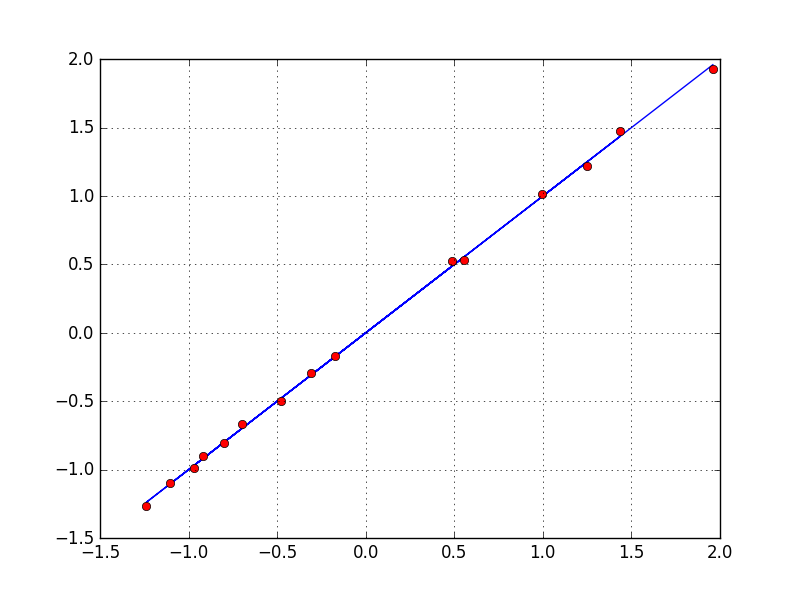
\includegraphics[scale=0.7]{figure_1.png}
   		\caption{Линейная регрессия}
   		\label{fig:im_1}
    \end{figure}
\end{center}

\vspace{0.5cm}
Расчётное значение критерия Фишера (F-критерий) равно $21562.733249157056$. Табличное значение критерия для уровня доверия $95\%$ равно $4.67$. Так как расчётный критерий много больше табличного, мы можем утверждать, что полученное уравнение регрессии статистически значимо.

\vspace{0.5cm}
Расчетное значение критерия Стьюдента для коэффициентов $a$ и $b$ равно\\ $3.7357497490332565$ и $1.2169545309210383e-15$ соответственно. Критическому значению t-критерия соответствует $2.16037$, таким образом можно утверждать, что параметр $b$ статистически незначим и им можно пренебречь, в отличии от параметра $a$.


\vspace{0.5cm}
Вычисленный коэффициент детерминации $R^2 = 0.9996986902215901$ означает, что изменение $X$ в $99,99\%$ случаев влечет за собой изменение $Y$.

\newpage\section{Параболическая регрессия}

Ниже представлена выборка в исходном и стандартизированном видах (таблица ~\ref{table:p}), а также параметры первой (таблица ~\ref{table:p_params})

\begin{table}[h]
	\caption{Выборка для параболической регресии}
	\begin{tabular}{*{4}{|c}|}
		\hline 
		$X$ Исходное & $Y$ Исходное & $X$ Стандартизированное & $Y$ Стандартизированное \\
		\hline
		0.83 & 14.65 & -0.658295 & -0.57669\\
		\hline
		4.7 & 152.1 & 1.034838 & 0.739438\\
		\hline
		3.46 & 92.27 & 0.492336 & 0.166547\\
		\hline
		0.07 & 2.82 & -0.990797 & -0.689966\\
		\hline
		0.8 & 14.0 & -0.67142 & -0.582914\\
		\hline
		8.58 & 416.15 & 2.732347 & 3.267802\\
		\hline
		0.4 & 7.49 & -0.846421 & -0.645249\\
		\hline
		2.05 & 43.76 & -0.124542 & -0.297952\\
		\hline
		4.8 & 155.84 & 1.078589 & 0.77525\\
		\hline
		1.69 & 34.17 & -0.282043 & -0.389779\\
		\hline
		0.54 & 9.71 & -0.785171 & -0.623992\\
		\hline
		3.82 & 110.14 & 0.649837 & 0.337658\\
		\hline
		2.29 & 50.53 & -0.019542 & -0.233127\\
		\hline
		0.84 & 15.1 & -0.65392 & -0.572381\\
		\hline
		0.15 & 4.42 & -0.955796 & -0.674645\\
		\hline
	\end{tabular} 
	\label{table:p}
\end{table}

\begin{table}[h]
	\caption{Характеристики исходной выборки}
	\begin{tabular}{|c|c|c|}
	\hline 
	Выборка & Мат. ожидание & Среднеквадратичное отклонение \\ 
	\hline 
	$X$ & 2.3346666666666667 & 2.285703003940412 \\ 
	\hline 
	$Y$ & 74.87666666666668 & 104.43514585085276 \\ 
	\hline 
	\end{tabular} 
	\label{table:p_params}
\end{table}

Применив метод наименьших квадратов получим такую систему линейных уравнений для определени параметров уравнения регрессии.

$$y = ax^2 + bx + c$$
$$F(a, b, c) = \sum\limits_{i=1}^n (ax_i^2 + bx_i + c - y_i)^2$$
$$\left\{
\begin{array}{l l}

\frac{\partial F(a, b, c)}{\partial a} = 2\sum\limits_{i=1}^n (ax_i^2 + bx_i + c - y_i)x_i^2 = a\ 2\sum\limits_{i=1}^n x_i^4 + b\ 2\sum\limits_{i=1}^n x_i^3 + c\ 2\sum\limits_{i=1}^n x_i^2 - 2\sum\limits_{i=1}^n x_i^2y_i\\

\frac{\partial F(a, b, c)}{\partial b} = 2\sum\limits_{i=1}^n (ax_i^2 + bx_i + c - y_i)x_i = a\ 2\sum\limits_{i=1}^n x_i^3 + b\ 2\sum\limits_{i=1}^n x_i^2 + c\ 2\sum\limits_{i=1}^n x_i - 2\sum\limits_{i=1}^n x_iy_i\\

\frac{\partial F(a, b, c)}{\partial c} = 2\sum\limits_{i=1}^n (ax_i^2 + bx_i + c - y_i) = a\ 2\sum\limits_{i=1}^n x_i^2 + b\ 2\sum\limits_{i=1}^n x_i + c\ 2n - 2\sum\limits_{i=1}^n y_i\\
\end{array}
\right.$$

Итоговое уравнение:
$$y = 0.2135817829018743*x^2+0.6909999979747826*x-0.21358178290187405$$

На графике представлена выборка в стандартизированном виде(красные точки) и уравнение регрессии (рис. \ref{fig:im_2}). 

\begin{center}
	\begin{figure}[h]
		\centering
   		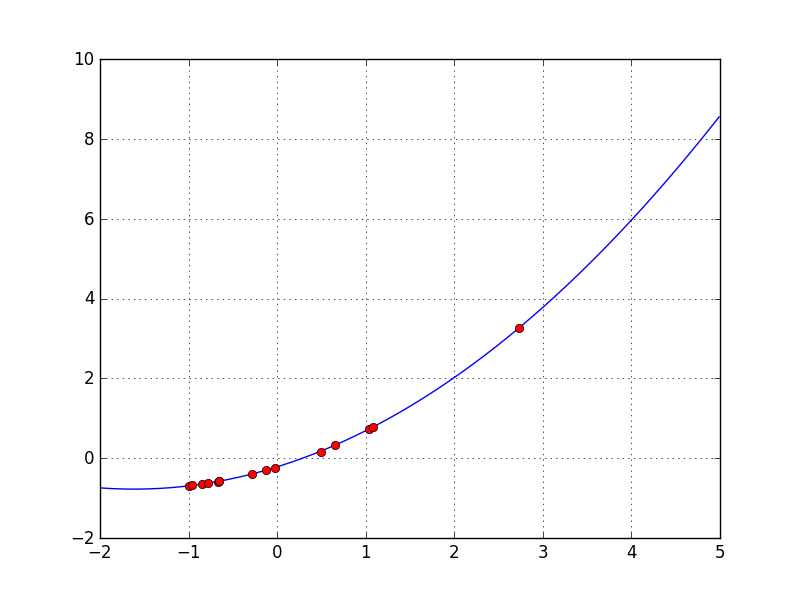
\includegraphics[scale=0.7]{figure_2.png}
   		\caption{Параболическая регрессия}
   		\label{fig:im_2}
    \end{figure}
\end{center}

\newpage\section{Множественная регрессия}

Ниже представлена выборка в исходном и стандартизированном видах (таблица ~\ref{table:m}), а также параметры первой (таблица ~\ref{table:m_params})

\begin{table}[h]
	\caption{Выборка для множественной регресии}
	\begin{tabular}{*{6}{|c}|}
	\hline 
	$X$ Исходное & $Y$ Исходное & $Z$ Исходное & $X$ Станд. & $Y$ Станд. & $Z$ Станд.\\
		\hline
		2.3 & 6.33 & 59.06 & -0.078401 & 1.285818 & 1.158237\\
		\hline
		3.33 & 0.03 & 15.79 & 1.170353 & -0.950696 & -0.558056\\
		\hline
		3.16 & 0.23 & 15.7 & 0.964248 & -0.879696 & -0.561626\\
		\hline
		2.43 & 0.15 & 8.81 & 0.079209 & -0.908096 & -0.834916\\
		\hline
		1.34 & 0.28 & 2.36 & -1.242288 & -0.861946 & -1.090754\\
		\hline
		1.68 & 1.17 & 11.51 & -0.830078 & -0.545994 & -0.727822\\
		\hline
		1.91 & 8.58 & 74.74 & -0.55123 & 2.084574 & 1.78018\\
		\hline
		3.54 & 5.29 & 61.22 & 1.424954 & 0.916616 & 1.243913\\
		\hline
		2.64 & 2.53 & 31.03 & 0.333809 & -0.06319 & 0.046434\\
		\hline
		3.42 & 2.59 & 35.02 & 1.279468 & -0.04189 & 0.204696\\
		\hline
		1.12 & 0.22 & 0.16 & -1.509012 & -0.883246 & -1.178016\\
		\hline
		1.94 & 1.89 & 20.75 & -0.514858 & -0.290392 & -0.361319\\
		\hline
		3.3 & 7.9 & 76.99 & 1.133982 & 1.843172 & 1.869426\\
		\hline
		1.05 & 1.08 & 6.81 & -1.593879 & -0.577944 & -0.914246\\
		\hline
		2.31 & 2.35 & 27.94 & -0.066277 & -0.127091 & -0.07613\\
		\hline
	\end{tabular} 
	\label{table:m}
\end{table}

\begin{table}[h]
	\caption{Характеристики исходной выборки}
	\begin{tabular}{|c|c|c|}
	\hline 
	Выборка & Мат. ожидание & Среднеквадратичное отклонение \\ 
	\hline 
	$X$ & 2.3646666666666665 & 0.8248221357089998 \\ 
	\hline 
	$Y$ & 2.708 & 2.816882910831285 \\ 
	\hline 
	$Z$ & 29.859333333333336 & 25.21130949042953 \\ 
	\hline 
	\end{tabular} 
	\label{table:m_params}
\end{table}

Применив метод наименьших квадратов получим такую систему линейных уравнений для определени параметров уравнения регрессии.

$$z = ax + by + c$$
$$F(a, b, c) = \sum\limits_{i=1}^n (ax_i + by_i + c - z_i)^2$$
$$\left\{
\begin{array}{l l}

\frac{\partial F(a, b, c)}{\partial a} = 2\sum\limits_{i=1}^n (ax_i + by_i + c - z_i)x_i = a\ 2\sum\limits_{i=1}^n x_i^2 + b\ 2\sum\limits_{i=1}^n x_iy_i + c\ 2\sum\limits_{i=1}^n x_i - 2\sum\limits_{i=1}^n x_iz_i\\

\frac{\partial F(a, b, c)}{\partial b} = 2\sum\limits_{i=1}^n (ax_i + by_i + c - z_i)y_i = a\ 2\sum\limits_{i=1}^n x_iy_i + b\ 2\sum\limits_{i=1}^n y_i^2 + c\ 2\sum\limits_{i=1}^n y_i - 2\sum\limits_{i=1}^n y_iz_i\\

\frac{\partial F(a, b, c)}{\partial c} = 2\sum\limits_{i=1}^n (ax_i + by_i + c - z_i) = a\ 2\sum\limits_{i=1}^n x_i + b\ 2\sum\limits_{i=1}^n y_i + c\ 2n - 2\sum\limits_{i=1}^n z_i\\
\end{array}
\right.$$
Итоговое уравнение:
$$z = 0.24084103100742218000*x + 0.90807086877838860000*y-0.00000000000000022177$$

\begin{center}
	\begin{figure}[h]
		\centering
   		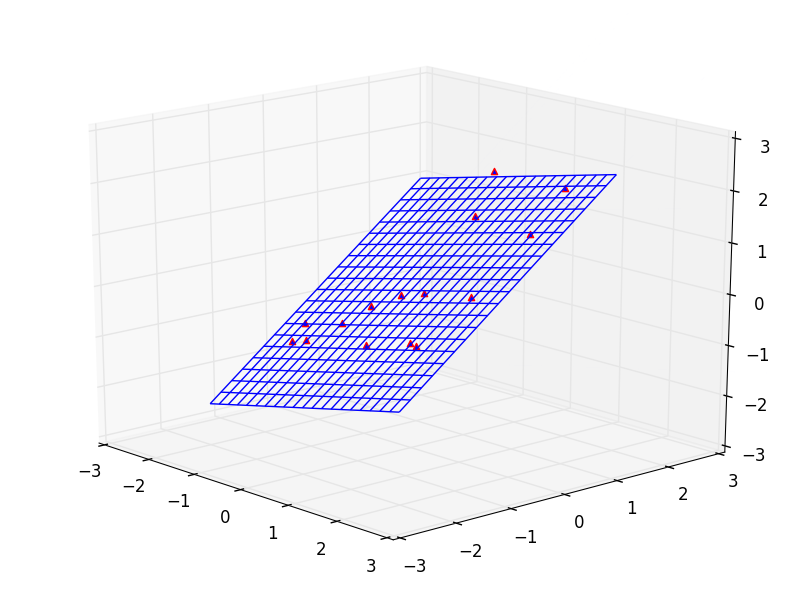
\includegraphics[scale=0.35]{figure_3-1.png}
   		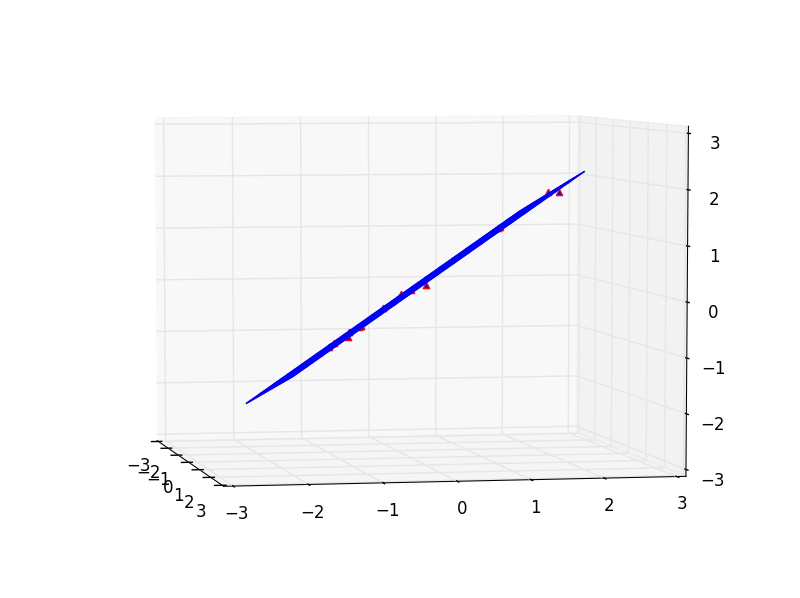
\includegraphics[scale=0.35]{figure_3-2.png}
   		\caption{Множественная регрессия}
   		\label{fig:im_3}
    \end{figure}
\end{center}

\newpage\section{Выводы}
Подводя общий итог можно сказать, что все модели достаточно точно описывают взяимосвязь между рассмотренными СВ и могут применяться для оценки данных за пределами эксперементальной выборки.

\newpage\section{Приложения}

\begin{lstlisting}[language=Java, title=Класс для вспомогательных вычислений]
package helpers;

import java.util.stream.DoubleStream;

/**
 * Класс для вспомогательных вычислений
 *
 * @author Roman
 */
public class CalculationHelper {

    /**
     * Метод для нормализации массива значений
     *
     * @param array массив значений
     * @return нормализованный массив
     */
    public static double[] normalizedArray(double[] array) {
        double expValue = calculateExpectedValue(array);
        double standartDeviation = calculateStandardDeviation(array);
        return DoubleStream.of(array).map(xi ->
                (xi - expValue) / standartDeviation
        ).toArray();
    }

    /**
     * Метод для подсчета стандартного отклонения для массива значений
     *
     * @param array массив значений
     * @return стандартное отклонение
     */
    private static double calculateStandardDeviation(double[] array) {
        return Math.sqrt(calculateDispersion(array));
    }

    /**
     * Метод для подсчета диссперсии для массива значений
     *
     * @param array массив значений
     * @return диссперсия
     */
    public static double calculateDispersion(double[] array) {
        double expValue = calculateExpectedValue(array);
        return calculateExpectedValue(
                DoubleStream.of(array)
                        .map(s -> Math.pow(s - expValue, 2))
                        .toArray()
        );
    }

    /**
     * Метод для подсчет математического ожидания для массива значений
     *
     * @param array массив значений
     * @return математическое ожидание
     */
    public static double calculateExpectedValue(double[] array) {
        return DoubleStream.of(array).sum() / array.length;
    }

    /**
     * Метод для подсчета коэффициента Фишера
     * нужен для анализа реграссии
     *
     * @param y    первоначальный массив нормализованных значений
     * @param newY новые значения Y, высчитаные по полученной формуле
     * @return коэффициент Фишера
     */
    public static double calculateCoefficientFisher(double[] y, 
    double[] newY) {
        double expValueY = CalculationHelper.calculateExpectedValue(y);
        double numerator = 0;
        double denominator = 0;
        for (int i = 0; i < y.length; i++) {
            numerator += Math.pow(newY[i] - expValueY, 2);
            denominator += Math.pow(y[i] - newY[i], 2) / (y.length - 2);
        }
        return numerator / denominator;
    }

    /**
     * Метод для высчитывания коэффициентов Стьюдента
     * @param a значение стоящее у переменной X в уравнении функции
     * @param b значение b в уравнениее функции
     * @param y массив значений Y
     * @param x массив значений X
     * @return коэффициенты Стьюдента
     */
    public static double[] calculateCoefficientStudent(double a, 
    double b, double[] y, double[] x) {
        double[] result = new double[2];
        double expValueY = calculateExpectedValue(y);
        double expValueX = calculateExpectedValue(x);
        double residualDispersionY = DoubleStream.of(y)
                .map(valuyY -> Math.pow(valuyY - expValueY, 2))
                .sum();
        residualDispersionY = Math.sqrt(residualDispersionY / (y.length - 2));
        double numeratorA = DoubleStream.of(x)
                .map(value -> Math.pow(value, 2))
                .sum();
        double denominatorA = DoubleStream.of(x)
                .map(value -> Math.pow(value - expValueX, 2))
                .sum();
        numeratorA *= residualDispersionY;
        denominatorA *= y.length;
        result[0] = a / Math.sqrt(numeratorA / denominatorA);

        double denominatorB = DoubleStream.of(x)
                .map(value -> Math.pow(value - expValueX, 2))
                .sum();
        result[1] = b / Math.sqrt(residualDispersionY / denominatorB);
        return result;
    }
}
\end{lstlisting}
\begin{lstlisting}[language=Java, title=Вспомогательный класс для вычисления различных видов регрессий]
package helpers;

import org.apache.commons.math.linear.RealVector;
import org.apache.commons.math.stat.regression.OLSMultipleLinearRegression;
import org.apache.commons.math.stat.regression.SimpleRegression;
import org.apache.commons.math3.fitting.PolynomialCurveFitter;
import org.apache.commons.math3.fitting.WeightedObservedPoints;

public class RegressionHelper extends OLSMultipleLinearRegression {
    /**
     * Метод для высчитывания коэффициентов параболической регрессии
     * @param arrayX массив значений X
     * @param arrayY массив значений Y
     * @return коэффициенты уравнения
     */
    public static double[] calculateCoefficientPolynomialRegression(
    double[] arrayX, double[] arrayY) {
        WeightedObservedPoints obs = new WeightedObservedPoints();
        for (int j = 0; j < arrayX.length; j++) {
            obs.add(arrayX[j], arrayY[j]);
        }
        PolynomialCurveFitter fitter = PolynomialCurveFitter.create(2);
        return fitter.fit(obs.toList());
    }

    /**
     * Метод для высчитывания коэффициентов множественной регрессии
     * @param z массив значений Z
     * @param data масив со значениям X и Y
     * @return коэффициенты уравнения
     */
    public static double[] calculateCoefficientMultipleRegression(
    double[] z, double[][] data) {
        RegressionHelper regressionHelper = new RegressionHelper();
        regressionHelper.newSampleData(z, data);
        RealVector vector = regressionHelper.calculateBeta();
        return vector.getData();
    }

    /**
     * Метод для получения линейной зависимости по vfccbdfv значений
     * @param x массив значений X
     * @param y массив значений Y
     * @return линейная регрессия
     */
    public static SimpleRegression getSimpleRegression(double[] x, 
    
    double[] y) {
        SimpleRegression regression = new SimpleRegression();
        for (int i = 0; i < x.length; i++) {
            regression.addData(x[i], y[i]);
        }
        return regression;
    }
}
\end{lstlisting}

\end{document}
